% ========================================
%	Header einbinden
% ========================================

\documentclass[bibtotoc,titlepage]{scrartcl}

% Deutsche Spracheinstellungen
\usepackage[ngerman,german]{babel, varioref}
\usepackage[T1]{fontenc}
\usepackage[utf8]{inputenc}

%\usepackage{marvosym}

\usepackage{amsfonts}
\usepackage{amssymb}
\usepackage{amsmath}
\usepackage{amscd}
\usepackage{amstext}
\usepackage{float}
\usepackage{caption}
\usepackage{wrapfig}
\usepackage{setspace}
\usepackage{threeparttable}
\usepackage{footnote}

\usepackage{caption}
\usepackage{subcaption}

\newfloat{formel}{htbp}{for}
\floatname{formel}{Formel}


\usepackage{longtable}

%\usepackage{bibgerm}

\usepackage{footnpag}

\usepackage{ifthen}                 %%% package for conditionals in TeX
\usepackage{siunitx}
%Fr textumflossene Bilder und Tablellen
%\usepackage{floatflt} - veraltet

%Fr Testzwecke aktivieren, zeigt labels und refs im Text an.
%\usepackage{showkeys}

% Abstand zwischen zwei Abs�zen nach DIN (1,5 Zeilen)
% \setlength{\parskip}{1.5ex plus0.5ex minus0.5ex}

% Einrckung am Anfang eines neuen Absatzes nach DIN (keine)
%\setlength{\parindent}{0pt}

% R�der definieren
% \setlength{\oddsidemargin}{0.3cm}
% \setlength{\textwidth}{15.6cm}

% bessere Bildunterschriften
%\usepackage[center]{caption2}


% Probleml�ungen beim Umgang mit Gleitumgebungen
\usepackage{float}

% Nummeriert bis zur Strukturstufe 3 (also <section>, <subsection> und <subsubsection>)
%\setcounter{secnumdepth}{3}

% Fhrt das Inhaltsverzeichnis bis zur Strukturstufe 3
%\setcounter{tocdepth}{3}

\usepackage{exscale}

\newenvironment{dsm} {\begin{displaymath}} {\end{displaymath}}
\newenvironment{vars} {\begin{center}\scriptsize} {\normalsize \end{center}}


\newcommand {\en} {\varepsilon_0}               % Epsilon-Null aus der Elektrodynamik
\newcommand {\lap} {\; \mathbf{\Delta}}         % Laplace-Operator
\newcommand {\R} { \mathbb{R} }                 % Menge der reellen Zahlen
\newcommand {\e} { \ \mathbf{e} }               % Eulersche Zahl
\renewcommand {\i} { \mathbf{i} }               % komplexe Zahl i
\newcommand {\N} { \mathbb{N} }                 % Menge der nat. Zahlen
\newcommand {\C} { \mathbb{C} }                 % Menge der kompl. Zahlen
\newcommand {\Z} { \mathbb{Z} }                 % Menge der kompl. Zahlen
\newcommand {\limi}[1]{\lim_{#1 \rightarrow \infty}} % Limes unendlich
\newcommand {\sumi}[1]{\sum_{#1=0}^\infty}
\newcommand {\rot} {\; \mathrm{rot} \,}         % Rotation
\newcommand {\grad} {\; \mathrm{grad} \,}       % Gradient
\newcommand {\dive} {\; \mathrm{div} \,}        % Divergenz
\newcommand {\dx} {\; \mathrm{d} }              % Differential d
\newcommand {\cotanh} {\; \mathrm{cotanh} \,}   %Cotangenshyperbolicus
\newcommand {\asinh} {\; \mathrm{areasinh} \,}  %Area-Sinus-Hyp.
\newcommand {\acosh} {\; \mathrm{areacosh} \,}  %Area-Cosinus-H.
\newcommand {\atanh} {\; \mathrm{areatanh} \,}  %Area Tangens-H.
\newcommand {\acoth} {\; \mathrm{areacoth} \,}  % Area-cotangens
\newcommand {\Sp} {\; \mathrm{Sp} \,}
\newcommand {\mbe} {\stackrel{\text{!}}{=}}     %Must Be Equal
\newcommand{\qed} { \hfill $\square$\\}
\renewcommand{\i} {\imath}
\def\captionsngerman{\def\figurename{\textbf{Abb.}}}

%%%%%%%%%%%%%%%%%%%%%%%%%%%%%%%%%%%%%%%%%%%%%%%%%%%%%%%%%%%%%%%%%%%%%%%%%%%%
% SWITCH FOR PDFLATEX or LATEX
%%%%%%%%%%%%%%%%%%%%%%%%%%%%%%%%%%%%%%%%%%%%%%%%%%%%%%%%%%%%%%%%%%%%%%%%%%%%
%%%
\ifx\pdfoutput\undefined %%%%%%%%%%%%%%%%%%%%%%%%%%%%%%%%%%%%%%%%% LATEX %%%
%%%
\usepackage[dvips]{graphicx}       %%% graphics for dvips
\DeclareGraphicsExtensions{.eps,.ps}   %%% standard extension for included graphics
\usepackage[ps2pdf]{thumbpdf}      %%% thumbnails for ps2pdf
\usepackage[ps2pdf,                %%% hyper-references for ps2pdf
bookmarks=true,%                   %%% generate bookmarks ...
bookmarksnumbered=true,%           %%% ... with numbers
hypertexnames=false,%              %%% needed for correct links to figures !!!
breaklinks=true,%                  %%% breaks lines, but links are very small
linkbordercolor={0 0 1},%          %%% blue frames around links
pdfborder={0 0 112.0}]{hyperref}%  %%% border-width of frames
%                                      will be multiplied with 0.009 by ps2pdf
%
%\hypersetup{ pdfauthor   = {Hannes Franke; Julius Tilly},
%pdftitle    = {x}, pdfsubject  = {Protokoll FP}, pdfkeywords = {V301, Innenwiderstand, Leistungsanpassung},
%pdfcreator  = {LaTeX with hyperref package}, pdfproducer = {dvips
%+ ps2pdf} }
%%%
\else %%%%%%%%%%%%%%%%%%%%%%%%%%%%%%%%%%%%%%%%%%%%%%%%%%%%%%%%%% PDFLATEX %%%
%%%
\usepackage[pdftex]{graphicx}      %%% graphics for pdfLaTeX
\DeclareGraphicsExtensions{.pdf}   %%% standard extension for included graphics
\usepackage[pdftex]{thumbpdf}      %%% thumbnails for pdflatex
\usepackage[pdftex,                %%% hyper-references for pdflatex
bookmarks=true,%                   %%% generate bookmarks ...
bookmarksnumbered=true,%           %%% ... with numbers
hypertexnames=false,%              %%% needed for correct links to figures !!!
breaklinks=true,%                  %%% break links if exceeding a single line
linkbordercolor={0 0 1},
linktocpage]{hyperref} %%% blue frames around links
%                                  %%% pdfborder={0 0 1} is the default
% \hypersetup{
% pdftitle    = {V301 Innenwiderstand und Leistungsanpassung}, 
% pdfsubject  = {Protokoll AP}, 
% pdfkeywords = {V301, Innenwiderstand, Leistungsanpassung},
% pdfsubject  = {Protokoll AP},
% pdfkeywords = {V301, Innenwiderstand, Leistungsanpassung}}
%                                  %%% pdfcreator, pdfproducer,
%                                      and CreationDate are automatically set
%                                      by pdflatex !!!
\pdfadjustspacing=1                %%% force LaTeX-like character spacing
\usepackage{epstopdf}
%
\fi %%%%%%%%%%%%%%%%%%%%%%%%%%%%%%%%%%%%%%%%%%%%%%%%%%% END OF CONDITION %%%
%%%%%%%%%%%%%%%%%%%%%%%%%%%%%%%%%%%%%%%%%%%%%%%%%%%%%%%%%%%%%%%%%%%%%%%%%%%%
% seitliche Tabellen und Abbildungen
%\usepackage{rotating}
\usepackage{ae}
\usepackage{
  array,
  booktabs,
  dcolumn
}
\makeatletter 
  \renewenvironment{figure}[1][] {% 
    \ifthenelse{\equal{#1}{}}{% 
      \@float{figure} 
    }{% 
      \@float{figure}[#1]% 
    }% 
    \centering 
  }{% 
    \end@float 
  } 
  \makeatother 


  \makeatletter 
  \renewenvironment{table}[1][] {% 
    \ifthenelse{\equal{#1}{}}{% 
      \@float{table} 
    }{% 
      \@float{table}[#1]% 
    }% 
    \centering 
  }{% 
    \end@float 
  } 
  \makeatother 
%\usepackage{listings}
%\lstloadlanguages{[Visual]Basic}
%\allowdisplaybreaks[1]
%\usepackage{hycap}
%\usepackage{fancyunits}
\usepackage{xfrac}
\renewcommand {\i} { \text{i} }

% ========================================
%	Angaben für das Titelblatt
% ========================================

\title{Molekül- und Ionendynamik in Festkörpern\\untersucht mit der Festkörper-NMR-Spektroskopie\\% Titel des Versuchs 
\large TU Dortmund, Fakultät Physik\\ 
\normalsize Fortgeschrittenen-Praktikum}

\author{Jan Adam\\			% Name Praktikumspartner A
{\small \href{jan.adam@tu-dortmund.de}{jan.adam@tu-dortmund.de}}	% Erzeugt interaktiven einen Link
\and						% um einen weiteren Author hinzuzfügen
Dimitrios Skodras\\					% Name Praktikumspartner B
{\small \href{dimitrios.skodras@tu-dortmund.de}{dimitrios.skodras@tu-dortmund.de}}		% Erzeugt interaktiven einen Link
}
\date{08. Mai 2015}				% Das Datum der Versuchsdurchführung

% ========================================
%	Das Dokument beginnt
% ========================================

\begin{document}

% ========================================
%	Titelblatt erzeugen
% ========================================

\maketitle					% Jetzt wird die Titelseite erzeugt
\thispagestyle{empty} 				% Weder Kopfzeile noch Fußzeile

% ========================================
%	Der Vorspann
% ========================================

%\newpage					% Wenn Verzeichnisse auf einer neuen Seite beginnen sollen
%\pagestyle{empty}				% Weder Kopf- noch Fußzeile für Verzeichnisse

\tableofcontents

%\newpage					% eine neue Seite
%\thispagestyle{empty}				% Weder Kopf- noch Fußzeile für Verzeichnisse
%\listoffigures					% Abbildungsverzeichnis

%\newpage					% eine neue Seite
%\thispagestyle{empty}				% Weder Kopf- noch Fußzeile für Verzeichnisse
%\listoftables					% Tabellenverzeichnis
\newpage					% eine neue Seite


% ========================================
%	Kapitel
% ========================================

%\section{Einleitung}				% Bei Bedarf
\setcounter{page}{1}
\section{Theorie}
\subsection{Kernmomente in äußeren Magnetfeldern}
Ziel des Versuchs ist es, die Relaxationszeiten $T_1$ und $T_2$ von Dimethylsulfon-Kristallen mit der Deuteron-NMR als Sonde zu errechnen. Mit diesen Werten
werden stimulierte Echos gemessen und die Korrelationszeit in Abhängigkeit von Evolutionszeit und Temperatur bestimmt.

\subsubsection{Einführung einiger Kenngrößen}
Eine charakteristische Größe für Atomkerne ist ihre Spinquantenzahl $I$, die ein magnetisches Moment $\mu$ induziert, abhängig von ihrem isotopenspezifischen
gyromagnetischen Faktors $\gamma$. Wirkt ein statisches äußeres Magnetfeld $B_0$ auf diesen Kernspin ergibt sich quantenmechanisch eine Aufspaltung der
Energieniveaus $E_m \propto - m \gamma B_0 = -m \omega_L $ mit $-I \leq m \leq +I$ als ganzen Zahl und $\omega_L$ der Larmorfrequenz. Dieser Effekt 
ist als Zeeman-Effekt bekannt. Hinzu kommt eine Aufspaltung der Niveaus durch die Wechselwirkung des Quadrupolmoments des Kerns mit einem elektrischen 
Feldgradienten. In Abbildung \ref{pic_deuteron} sind die beiden Aufspaltungseffekte für ein $I=1$ Teilchen, wie das Deuteron dargestellt.

\begin{figure}[H]
 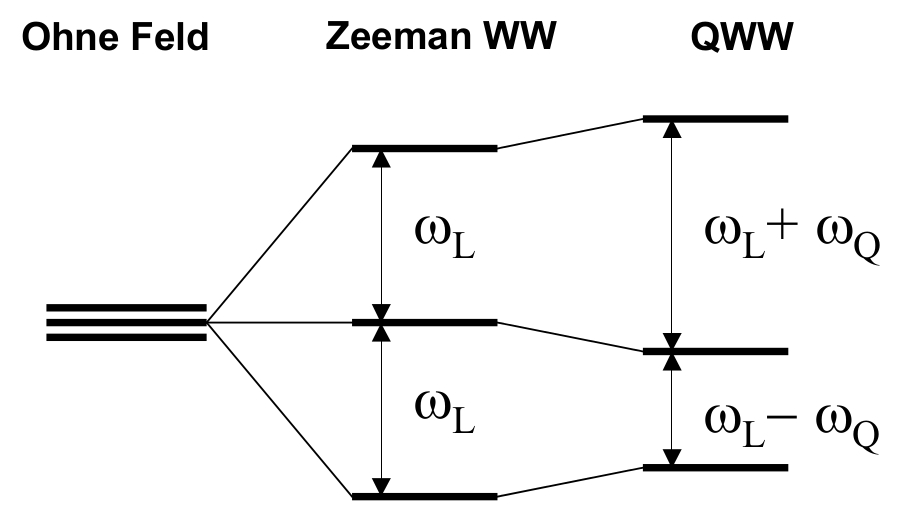
\includegraphics[width=0.4\textwidth]{../pics/deuteron.jpg}
 \caption{Niveauaufspaltungen durch Zeeman-Effekt und Quadrupolwechsewirkung eines Spin-1-Teilchens}
 \label{pic_deuteron}
\end{figure}

\noindent 
Im thermodynamischen Gleichgewicht sind diese Niveaus nach der Boltzmann-Verteilung besetzt, was zur makroskopischen Magnetisierung der Probe führt. Analog
zur Ausweichbewegung eines rotierenden Kreisels im Gravitationsfeld erfolgt eine Präzessionsbewegung der Kernspins im Magnetfeld mit der Frequenz 
$\omega_L =\gamma B_0$. Hierbei steht das Drehmoment $L\propto \sfrac{\dx I}{\dx t}$ senkrecht auf $B_0$ und $\mu$, was sich schreiben lässt als 
\begin{align}
 \frac{\dx \mu}{\dx t} = \gamma \mu \times B_0.
 \label{eq_dglMu}
\end{align}
Da $\vec B_0 = B_0 \textbf{e}_z$, zeigt auch die makroskopische Magnetisierung $M$ in $z$-Richtung, da die $x$- und $y$-Komponenten sich kompensieren, sodass
\eqref{eq_dglMu} auch hierfür anwenden lässt
\begin{align}
 \frac{\dx M}{\dx t} = \gamma M \times B_0.
 \label{eq_dglMagnetisierung}
\end{align}

\subsubsection{Einfluss von Hochfrequenzspulen}
\label{sec_hochfrequenz}
Beim Übergang auf zeitlich veränderliche, äußere Magnetfelder $B_1(t)$ ist die Transformation in ein sich mit $\Omega$ um die $z$-Achse rotierendes 
Koordinatensystem rechnerisch einfach zu handhaben. Die beiden Felder können dadurch in ein effektives Magnetfeld $B_\text{eff} = B_1 + B_0$ überführt
und \eqref{eq_dglMagnetisierung} damit geschrieben werden. Im Fall $\Omega$ = $\omega_L$ verschwindet das effektive Feld. Explizit im Laborsystem wird
das HF-Feld durch $B_1(t) = B_x \cos(\Omega t)$ gegeben. Dieses wird in zwei Komponenten entsprechend Abbildung \ref{pic_rotSystem} aufgeteilt, die mit
$\Omega$ gegenläufig rotieren. Die Komponente $B_\text{rechts}$ wird nun festgehalten und die andere läuft nun mit $-2\Omega$, die vernachlässigbar wird,
da sie von der Larmorfrequenz zu weit entfernt ist. Die Kernspins rotieren nun gleich mit $B_\text{rechts}$ und nehmen dieses als konstantes Feld mit 
Amplitude $B_x /2$ wahr. Bei anfänglicher Längsmagnetisierung entlang $z$, ergibt sich eine Präzessionsbewegung um die tranformierte $x$-Achse mit der
Rabi-Frequenz $\omega_1 = \gamma |B_\text{eff}|$.
\begin{figure}[H]
 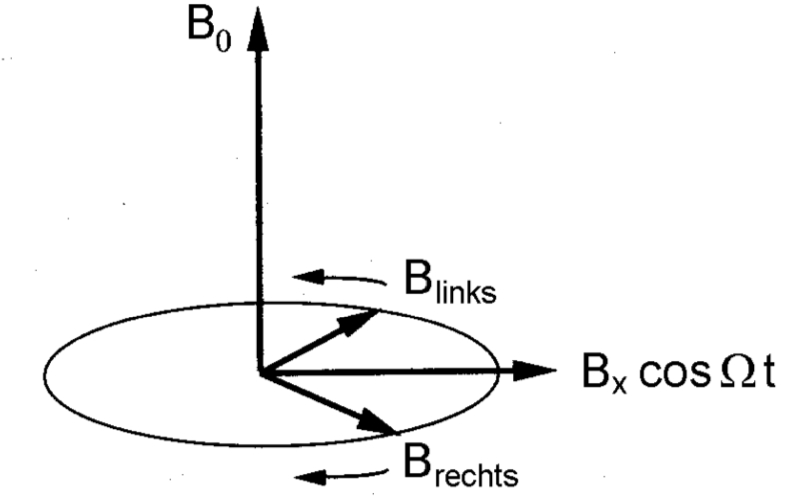
\includegraphics[width=0.4\textwidth]{../pics/rotSystem.jpg}
 \caption{Zerlegung des HF-Felds}
 \label{pic_rotSystem}
\end{figure}
\noindent
Wird dieses HF-Feld nun für eine gewisse Zeit eingeschaltet, wird der Magnetisierungsvektor um einen bestimmten Winkel $\alpha$ gedreht. Eine Drehung um
90$^\circ$ wird ($\pi$/2)-Puls genannt. Bei Anwesenheit des statischen $B_0$-Feldes induziert die Quermagnetisierung durch Präzession eine Spannung, das
Kerninduktionssignal, die mit einer Spule gemessen werden kann. Diese Quermagnetisierung verkleinert sich, was auch auf lokale Inhomogenitäten des 
Magnetfelds und dadurch auf verschiedene Larmorfrequenzen zurückführbar ist. Spinpakete mit gleichem $\omega_L$, genannt Isochromaten, rotieren schneller
oder langsamer als andere, was zur Dephasierung und damit zum Verschwinden der Quermagnetisierung führt. Dieser Prozess ist jedoch reversibel durch 
Einstrahlen eines ($\pi$)-Pulses, was in Abbildung \ref{pic_rephasierung} anschaulich wird. Zu Beginn wird ein ($\pi$/2)-Puls durchgeführt, woraufhin die
Spins präzedieren und dephasieren. Der ($\pi$)-Puls erhält den Drehsinn und die Drehgeschwindigkeit, wodurch die Spins rephasieren. Das schließliche 
Zusammentreffen wird Hahn-Echo bezeichnet.

\begin{figure}[t]
 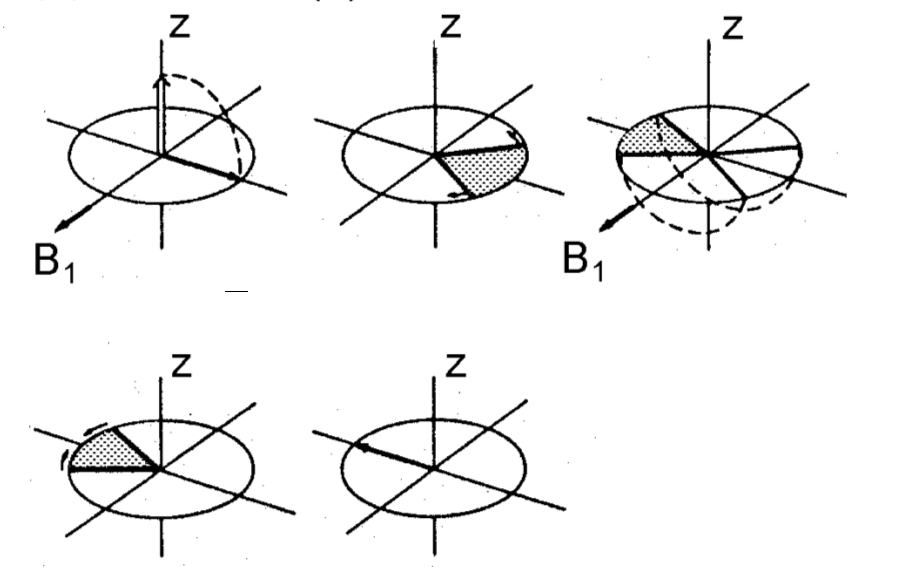
\includegraphics[width=0.6\textwidth]{../pics/rephasierung.jpg}
 \caption{Erzeugung von Quermagnetisierung, Dephasierung, $\pi$-Puls und Hahn-Echo}
 \label{pic_rephasierung}
\end{figure}

\subsection{Relaxation}
Die durch den HF-Puls kreierte Magnetisierung strebt ihrem Gleichgewichtszustand $M_\text{eq}$ durch Wechselwirkung der Spins mit ihrer Umgebung, auch
Gitter genannt. Die Längs- und Querkomponenten der Magnetisierung werden hierbei getrennt betrachtet
\begin{align}
 \frac{\dx M_z}{\dx t} &= -\frac{M_z(t) - M_\text{eq}}{T_1}\\
 \frac{\dx M_x}{\dx t} &= -\frac{M_x}{T_2}\\
 \frac{\dx M_y}{\dx t} &= -\frac{M_y}{T_2}
\end{align}
\noindent
Die longitudinale Komponente $M_z$ relaxiert durch Spin-Gitter Effekte mit $T_1$. Die transversalen Komponenten relaxieren durch Spin-Spin Effekte mit
$T_2$.

\subsubsection{Spin-Gitter-Relaxation}
Durch den ($\pi$)-Puls entsteht eine Besetzungsinversion entgegen der Boltzmann-Verteilung. Das thermische Gleichgewicht stellt sich durch Übergänge zwischen
den Niveaus neu ein, was in der Größenordnung von $T_1$ geschieht. Jedoch passiert das in diesem Frequenzbereich weniger durch spontane Emission, sondern durch 
magnetische Wechselfelder mit der Larmorfrequenz im Wesentlichen, die die Emission bedingt. Diese Inversionserholung kommt von stochastischen Bewegungen
der Spins, die zu zeitlich fluktuierenden Magnetfeldern führt. Die Fouriertransformierte davon, die Spektraldichte $J(\omega)$ gibt die Wahrscheinlichkeit an,
das ein Wechselfeld mit $\omega$ vorkommt. Je größer $J(\omega_L)$, umso effizienter der Kernspinübergang und damit $T_1$ auch. $T_1$ wird dann minimal, 
wenn Larmorfrequenz und Korrelationszeit $\tau_c$ einander entsprechen - $\omega_L \tau_c \approx 1$

\subsubsection{Spin-Spin-Relaxation}
Maßgeblich für diesen Prozess ist die magnetische Dipol-Dipol-Wechselwirkung, wobei die Spins einerseits selbst ein Magnetfeld erzeugen, aber auch bei anderen
Spins abhängig vom Winkel zwischen der Momentausrichtung und der internuklearen Verbindungslinie zueinander. Bei einem Festkörper sollten die Spins statisch 
verteilt sein, weshalb eine breite Verteilung lokaler Zusatzfelder und damit ein breiter Frequenzbereich für Resonanzabsorbtion zu erwarten ist. Bei
einfachen Flüssigkeiten mitteln sich die Zusatzfelder durch Molekularbewegungen auf experimentellen Zeitskalen hinaus, sodass nur noch bei der Larmorfrequenz
Resonanzabsorbtion auftritt. Hierbei erzeugte Quermagnetisierung relaxiert wenig, was einem langen $T_2$ entspricht.

\subsection{Untersuchungsmethoden}
Durch die Rephasierung der Isochromaten, also die Wiederherstellung der makroskopischen Magnetisierung, entsteht ein messbares Echo. Die verschiedenen 
Möglichkeiten, ein solches herzustellen geschieht durch die charakterisierenden Sequenzen. So das einfache Hahn-Echo, angesprochen in Abschnitt 
\ref{sec_hochfrequenz} und die hier Anwendung findenden Festkörperechos und die stimulierten Echos.
\subsubsection{Festkörperechos}
Festkörperechos sind im Gegensatz zu Hahn-Echos nützlich zur Refokussierung von Wechselwirkungen, die bilinear in den homonuklearen Spinoperatoren sind, wie
zum Beispiel der Säkularanteil der Dipolwechselwirkung oder der Spinanteil der Quadrupolwechsewirkung 1. Ordnung. Der ($\pi$)-Puls des Hahn-Echos ändert den
Hamiltonian nicht, wohingegen die Sequenz des Festkörperechos (vgl. Abb.) \ref{pic_festEchoFolge} das erreicht. Zu Beginn ein ($\pi/2$)$_x$-Puls und wartet
eine Zeit $\tau$, worauf ein ($\pi/2$)$_y$-Puls folgt, der um 90$^\circ$ zum vorigen phasenverschoben sein soll. Nach einer weiteren Wartezeit $\tau$ ist das
Echo messbar. 
\begin{figure}[htbp]
 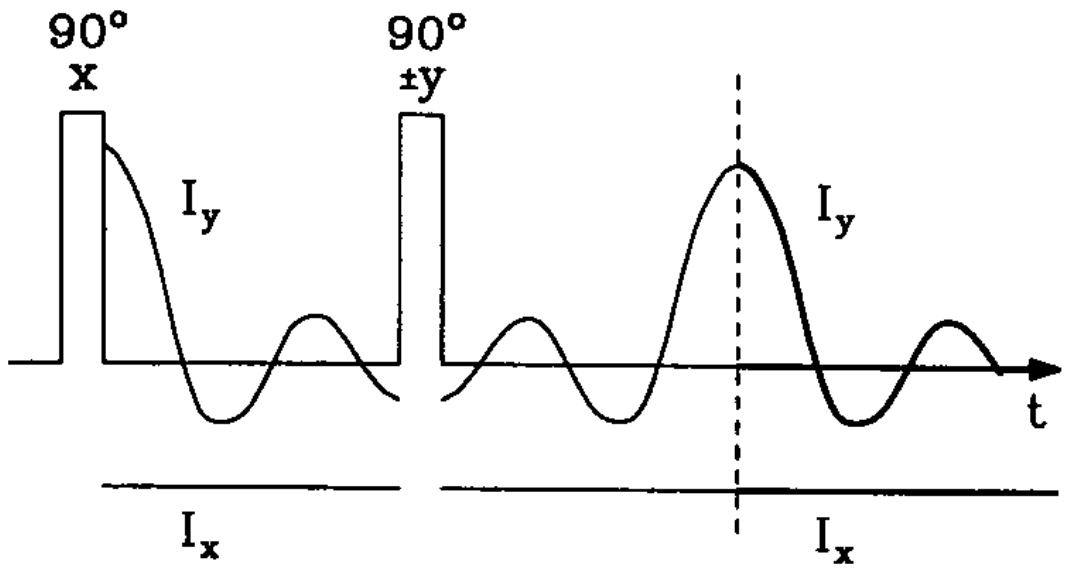
\includegraphics[width=0.5\textwidth]{../pics/festEchoFolge.jpg}
 \caption{Pulsfolge des Festkörperechos}
 \label{pic_festEchoFolge}
\end{figure}
\noindent

\subsubsection{Stimulierte Echos}
Für Prozesse, die für die Anwendung des Hahn-Echos zu langsam sind, muss das Depha-sierungs- und das Rephasierungsintervall getrennt werden. Der ($\pi$)-Puls
aus dem Hahn-Echo wird unterteilt in zwei Sequenzen. So wird zu Beginn ein ($\pi/2$)-Puls gegeben, um transversale Magnetisierung mit Amplitude $M_0$ zu
erzeugen (vgl. Abb. \ref{pic_stimEchoFolge}) . Die Spins dephasieren in der Zeit $t_1$ und entwickeln eine Phase zueinander. Der zweite Puls kann nun den 
$\cos$- oder den $\sin$-Anteil wieder zurückklappen. Dieser wird Speicherpuls genannt, da die longitudinale Magnetisierung mit $T_1$ relaxiert, während
der andere während der anschließenden Mischzeit $t_m$ dephasiert und die transversale Magnetisierung verschwindet. Schließlich kann ein dritter Puls den
gespeicherten Anteil in die Nachweisebene klappen. Die rephasierenden Spins erzeugen nach einer Zeit $t_2 = t_1$ ein Echo beispielsweise für den $\cos$-Anteil,
welches stimuliertes Echo bezeichnet wird. Die verbliebene Magnetisierung entspricht maximal der Hälfte von $M_0$. Bei chemischem Austausch sinkt dieser
Maximalwert auf der Zeitskala der Korrelationszeit. Daher lässt sich $\tau_c$ ermitteln aus der Echohöhe als Funktion der Mischzeit. Die stimulierten 
Echosignale $\langle\cos(\omega_1t_1)\cos(\omega_2t_2)\rangle$ und $\langle\sin(\omega_1t_1)\sin(\omega_2t_2)\rangle$ können für $t_1=t_2=t_p$ zu
$S(t_p,t_m) \sim \langle\exp(\i\omega_1t_p)\exp(-\i\omega_2t_p)\rangle$ zusammengefasst werden. Die $\omega_i$ sind zwei Präzessionsfrequenzen, $t_p$ die
Evolutionszeit.

\begin{figure}[H]
 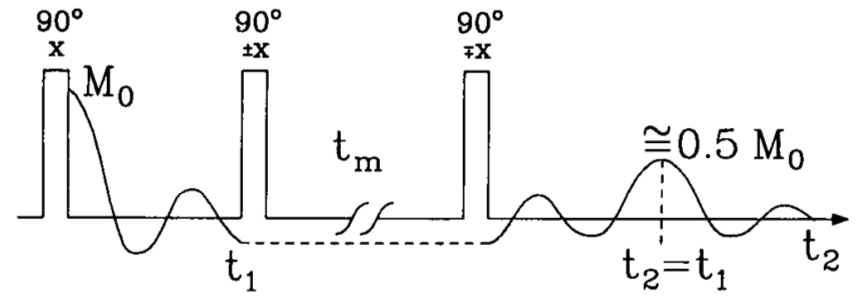
\includegraphics[width=0.6\textwidth]{../pics/stimEchoFolge.jpg}
 \caption{Pulsfolge des stimulierten Echos}
 \label{pic_stimEchoFolge}
\end{figure}
\noindent
Der Stoff Rb$_3$D(SO$_4$)$_2$ ist ein Ionenleiter, bei dem Deuteronen von Gitterplatz zu Gitterplatz kommen. Ein einem Einkristall davon gibt es zwei
unterscheidbare elektrische Feldgradienten beim Deuteron bzw. bei einer Leerstelle. Findet ein Sprung statt, ändert sich die NMR-Frequenz, was nachgewiesen
werden kann. Während relativ langer Mischzeiten können Deuteronen in die Leerstellen springen. Hierbei kann sich im Allgemeinen 
die Umgebung der Spins und damit die Präzessionsfrequenz ändern. Findet ein Sprung statt, entwickelt sich die Magnetisierung nach dem dritten Puls mit der
neuen Frequenz. Je mehr Sprünge stattfinden, bei beispielsweise längerer Mischzeit, entwickelt sich ein immer größerer Teil der Magnetisierung mit der 
neuen Frequenz, was in Abbildung \ref{pic_neueFrequenz} dargestellt ist.
\begin{figure}[H]
 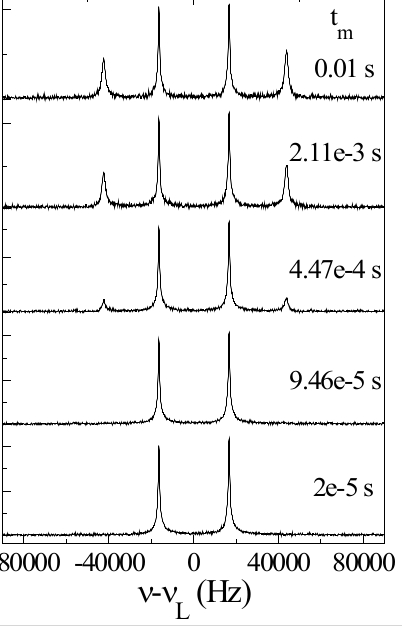
\includegraphics[width=0.3\textwidth]{../pics/neueFrequenz.jpg}
 \caption{$t_m$-abhängige Austauschintensität}
 \label{pic_neueFrequenz}
\end{figure}
\subsection{Korrelationszeit}
Die Funktion $S(t_p,t_m)$ ist analog zur inkohärenten, intermediären Streufunktion 
$S(q,t) \sim \langle\exp(\i\vec q \vec r(t))\exp(-\i\vec q \vec r(0))\rangle$, die messbar ist. $\vec q$ ist der Streuvektor und $\vec r$ der Ortsvektor. Für
hohe Phasendifferenzen zu erreichen, muss $\vec q$ oder $|\vec r(0)-\vec r(t)|$ bzw. $t_p$ oder $(\omega_1-\omega_2)$ groß sein. Dann findet man $\tau \approx$
const. Beispielhaft an K$_3$D(SO$_4$)$_2$ sind NMR-Messungen in Abbildung \ref{pic_tau(tp)} gezeigt. Die Korrelationszeit ist praktisch unabhängig von $t_p$,
was an der Kristallstruktur und den elektrischen Feldgradienten der Deuteronen plausibel wird.
\begin{figure}[H]
 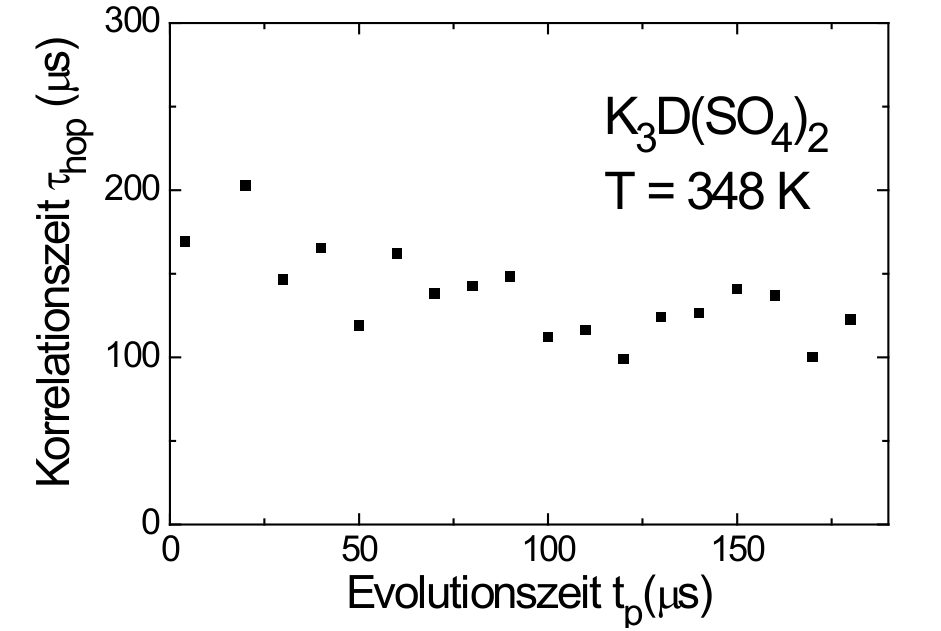
\includegraphics[width=0.4\textwidth]{../pics/tau(tp).jpg}
 \caption{$\tau_c$ als Funktion der Evolutionszeit $t_p$}
 \label{pic_tau(tp)}
\end{figure}
\noindent
Wenn die Deuteronen hüpfen, überwinden sie die Energiebarriere $E$ des Kristallfeldes durch thermischen Energie von $E \propto T$ mit einer Wahrscheinlichkeit
von $\Gamma = \Gamma_0 \exp(-\sfrac{E}{k_bT})$. Dabei ist $\Gamma_0$ die Anklopffrequenz, mit der das Ion an die Potentialbarriere stößt. mit 
$\tau = \Gamma^{-1}$ ergibt sich das Arrhenius-Gesetz
\begin{align}
 \tau = \tau_0 \exp \left(-\frac{E}{k_BT}\right).
 \label{eq_korrelationszeit}
\end{align}
In Abbildung \ref{pic_tau(T)} sind hier NMR-Messungen für Rb$_3$D(SO$_4$)$_2$ und K$_3$D(SO$_4$)$_2$ zu sehen. Die unterschiedlichen Steigungen entsprechen
verschiedenen Energiebarrieren.

\begin{figure}[H]
 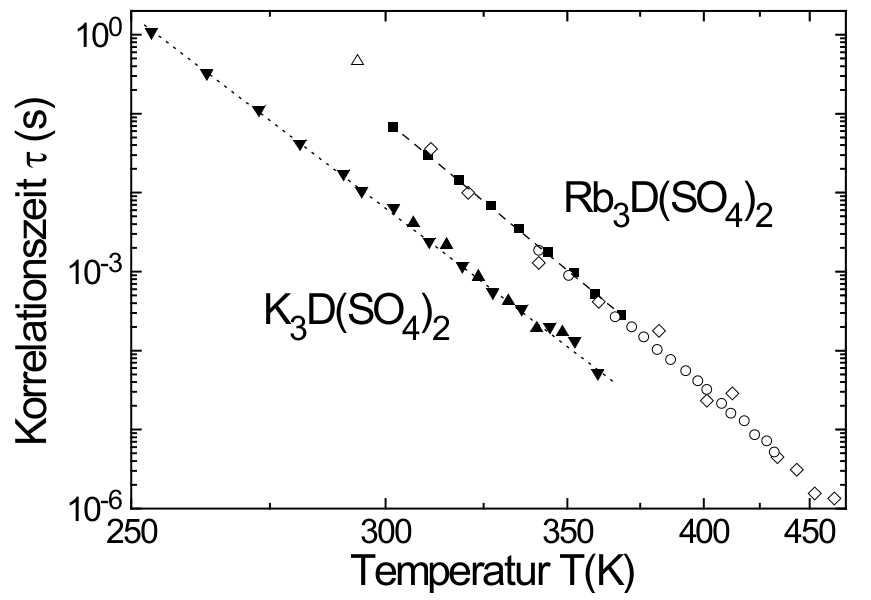
\includegraphics[width=0.4\textwidth]{../pics/tau(T).jpg}
 \caption{$\tau_c$ als Funktion der Temperatur $T$}
 \label{pic_tau(T)}
\end{figure}

\section{Aufbau und Durchführung}
Das NMR-Spektrometer erfüllt hier zwei Aufgaben. Die Manipulation des Spinsystems, sowie die Detektion des Kerninduktionssignals. Das Spinsystem wird durch
Magnetfelder gestört, welche durch Signale des HF-Generators induziert werden. Um starke Felder zu erzeugen, muss viel Leistung in den Probenstab gelangen,
was über ein Diodenpärchen am Ende des $\lambda$/4-Kabels ermöglicht wird. Das Diodenpaar ist gesperrt, wenn die Detektion läuft, sodass das Kerninduktionssignal
zum Vorverstärker gelangt. Dieses Signal $\omega_\text{RF}$ lässt sich nicht gut direkt messen, die Differenz davon mit $\omega_L$ jedoch schon. Daher wird
eine Quadraturdetekion durchgeführt, bei der das Kernsignal auch mit einem um 90$^\circ$ verschobenen Signal gemischt wird. Der Probenkopf besteht im Grunde
aus einem Reihenresonanzkreis, der auf die Larmorfrequenz abgestimmt ist, mit einer auf 50 $\Omega$ angepassten Impedanz. Die Impedanzanpassung vermeidet die 
Reflektion der eingestrahlen Welle und ist vor jeder Messung notwendig. Für die Anpassung wird ein Netzwerkanalysator verwendet für die Ausmessung des
Stehwellenverhältnisses VSWR, welches ein Maß für den Anteil der reflektierten Leistung ist.

\noindent Zu Beginn soll der Schwingkreis auf eine Resonanzfrequenz von 46,223 MHz eingestellt werden. Die Dauer eines $(\pi)$-Pulses soll mit einem 
Festkörperecho am Dimethylsulfon gemessen werden. $T_1$ wird durch eine saturation-recovery Messung bestimmt. Die Magnetisierung $M(t)$ soll mit einer
Kohlrauschfunktion $\propto \exp[-(t/T_1)^{1-\nu}]$ angepasst werden. $T_2$ wird mit einem Festkörperecho ermittelt. Mit diesen Werten werden die Einstellungen
für die stimulierten Echos festgesetzt. Bei einem bestimmten $t_p$ soll die Echohöhe in Abhängigkeit von $t_m$ gemessen werden. Die um $M(t)$ korrigierten
Echoamplituden werden mit einer weiteren Kohlrauschfunktion gefittet. Schließlich wird die Temperatur zweimal variiert und erneut stimulierte Echos für eine einzige
Präparationszeit gemessen.

\section{Auswertung}
\subsection{$T_1$ Messung}
Zunächst wird die $T_1$ Spin-Gitter Relaxationszeit mit der saturation-recovery Messung bei verschiedenen Probentemperaturen berechnet. Die dabei gemessenen Amplituden und Zeiten sind in Abb. \ref{pic_T1_hoch} und \ref{pic_T1_tief} dargestellt. 
\begin{figure}[htbp]
	\includegraphics[width=0.6\textwidth]{../auswertung/T1/T1_hochTemperaturFit.pdf}
	\caption{Amplituden als Funktion der Zeit}
	\label{pic_T1_hoch}
\end{figure}
\begin{figure}[htbp]
	\includegraphics[width=0.8\textwidth]{../auswertung/T1/T1_tiefTemperaturFit.pdf}
	\caption{Amplituden als Funktion der Zeit}
	\label{pic_T1_tief}
\end{figure}

Eine Regressionsfunktion der Form 
\begin{align}
	f(t) = A\cdot e^{-\left(\frac{t}{T_1}\right)^\nu}+c
\end{align}
\begin{table}[htbp]
	\begin{tabular}{| >{$}c<{$} | >{$}c<{$} | >{$}c<{$} |}
		\input{../auswertung/T1/T1_valuesHoch_table}
	\end{tabular}
	\caption{Temperaturen und gefittete $T_1$ Werte des Hochtemperaturbereiches.}
	\label{tab:T1_hoch}
\end{table}
\begin{table}[htbp]
	\begin{tabular}{| >{$}c<{$} | >{$}c<{$} | >{$}c<{$} |}
		\input{../auswertung/T1/T1_valuesTief_table}
	\end{tabular}
	\caption{Temperaturen und gefittete $T_1$ Werte des Tieftemperaturbereiches.}
	\label{tab:T1_tief}
\end{table}
wurde an die einzelne Messreihen angenähert und so für verschiedene Temperaturen die Relaxationszeit $T_1$ bestimmt. Die Ergebnisse der Fits stehen in Tabellen \ref{tab:T1_hoch} und \ref{tab:T1_tief}.

Diese T1 Werte können nun zusammen mit den entsprechenden Probentemperaturen in Arrhenius-Plots dargestellt werden. Zu sehen ist das Ergebnis in Abb. \ref{pic_T1Arr_hoch} und \ref{pic_T1Arr_tief}.
\begin{figure}[htbp]
	\includegraphics[width=0.8\textwidth]{../auswertung/T1/T1_hochTemperaturPlot.pdf}
	\caption{Arrhenius Plot der T1 Werte des Hochtemperaturbereiches.}
	\label{pic_T1Arr_hoch}
\end{figure}
\begin{figure}[htbp]
	\includegraphics[width=0.8\textwidth]{../auswertung/T1/T1_tiefTemperaturPlot.pdf}
	\caption{Arrhenius Plot der T1 Werte des Tieftemperaturbereiches.}
	\label{pic_T1Arr_tief}
\end{figure}

Im Hochtemperaturbereich ist hierbei die Position des Minimus von Bedeutung. Dieses wird durch den Fit einer quadratischen Funktion der Form:
\begin{align}
	g(x) = a(x-b)^2+c
\end{align}
bestimmt. Für die Position des Minimus ergibt sich:
\begin{align*}
	\input{../auswertung/T1/minimum.output}
\end{align*}

\newpage
\subsection{$T_2$ Messung}
Die Spin-Spin Relaxationszeit $T_2$ wird mit Hilfe eines Festkörperechos bestimmt. Dazu wird sowohl im Hoch- als auch im Tieftemperaturbereich die Echoamplitude gegen die Zeit aufgetragen. Die gemessenen Wertepaare sind in Abb. \ref{pic_T2_hoch} und \ref{pic_T2_tief} eingezeichnet.
\begin{figure}[htbp]
	\includegraphics[width=0.58\textwidth]{../auswertung/T2/T2_hochTemperaturFit.pdf}
	\caption{Festkörperecho Amplituden als Funktion der Zeit im Hochtemperaturbereich.}
	\label{pic_T2_hoch}
\end{figure}
\begin{figure}[htbp]
	\includegraphics[width=0.58\textwidth]{../auswertung/T2/T2_tiefTemperaturFit.pdf}
	\caption{Festkörperecho Amplituden als Funktion der Zeit im Tieftemperaturbereich.}
	\label{pic_T2_tief}
\end{figure}

Im Tieftemperaturbereich wurde eine Fitfunktion der Form
\begin{align}
	f(t) = \left[ M_\tau+(M_{Z_0}-M_\tau)\cdot e^{-\left(\frac{t}{T_{21}}\right)^{\beta_\tau}} \right] \cdot e^{-\left(\frac{t}{T_{22}}\right)^{\beta_{T_1}}}+M_0
\end{align}
an die Datenreihen angepasst. Die Ergebnisse des Fits sind in Tabelle aufgeführt.
\begin{table}[htbp]
	\begin{tabular}{| >{$}c<{$} | >{$}c<{$} | >{$}c<{$} |>{$}c<{$} | >{$}c<{$} |}
		\input{../auswertung/T2/T2_data_latex}
	\end{tabular}
	\caption{Temperaturen und gefittete $T_{21}$ und $T_{22}$ Werte des Tieftemperaturbereiches.}
	\label{tab:T1_tief}
\end{table}


\newpage
\subsection{$F_2$ Messung}
Um die $\tau_C$ Korrelationszeit zu bestimmen, wird die Echoamplitude in einem Plot gegen die Zeit aufgetragen und anschließend im Tieftemperaturbereich eine Funktion folgender Form angefittet:
\begin{align}
	h(t) = \left[M_\tau+(M_{z0}-M_\tau)\cdot e^{-\left(\frac{t}{T_c}\right)^{\beta_1}}\right]\cdot e^{-\left(\frac{t}{T_1}\right)^{\beta_2}}+M_0
\end{align}
\begin{figure}[htbp]
	\includegraphics[width=0.8\textwidth]{../auswertung/F2/F2_Plot.pdf}
	\caption{Arrhenius Plot der F2 Werte des Tieftemperaturbereiches.}
	\label{pic_F2_tief}
\end{figure}
Die Darstellung der Messwerte, sowie die Fitfunktionen ist in Abb. \ref{pic_F2_tief} sichtbar. Der Fit ergab für $\tau_c$ die in Tabelle \ref{tab:F2_tief} stehenden Werte.
\begin{table}[htbp]
	\begin{tabular}{| >{$}c<{$} | >{$}c<{$} | >{$}c<{$} |}
		\textbf{Temperatur }[K] & \tau_C & \text{Standardabweichung}\\\hline
		\input{../auswertung/F2/tauC_values_table}
	\end{tabular}
	\caption{Ergebnisse des Fits aus Abb. \ref{pic_F2_tief}.}
	\label{tab:F2_tief}
\end{table}

Trägt man diese Werte und ihre korrelierenden Temperaturen in einem Arrhenius-Plot wie in Abb. \ref{pic_F2_fit} auf, so kann aus der Steigung der Ausgleichsgeraden die Aktivierungsenergie $E_A$ bestimmt werden. 
Die Fit-Funktion ist:
\begin{align}
	g(T) = A\cdot e^{-\frac{E_A}{k_BT}}
\end{align}
und entspricht einer Geradengleichung in der Darstellung des Arrhenius-Plots.
\begin{figure}[htbp]
	\includegraphics[width=0.8\textwidth]{../auswertung/F2/F2_Plot.pdf}
	\caption{Arrhenius Plot der $\tau_C$ Werte des Tieftemperaturbereiches und Regressionsgerade. Die Steigung der Geraden entspricht der Aktivierungsenergie.}
	\label{pic_F2_fit}
\end{figure}
Für die Aktivierungsenergie $E_A$ ergab der Fit folgenden Wert: 
\begin{align}
	\input{../auswertung/F2/Ea.output}
\end{align}

\section{Diskussion}
Die $T_1$ Messreihen passen sehr gut mit den gefitteten Theoriekurven überein und die Fehler der daraus bestimmten Parameter sind um einen Faktor $10^{-2}$ kleiner als die Parameter selbst.
Die $T_1$ Arrheniusplots haben ebenfalls die Form, die im Hoch- bzw. Tieftemperaturbereich erwartet werden: Im Tieftemperaturbereich liegen die Werte auf einer Geraden (siehe Abb. \ref{pic_T1Arr_tief}) während die Werte im Hochtemperaturbereich ein Minimum ausbilden (siehe Abb. \ref{pic_T1Arr_hoch}).

Messungen der Spin-Spin Relaxationszeit $T_2$ sind mit einem Fehler, der um einen Faktor $10^{-4}$ kleiner als die Messwerte sind, sogar noch genauer als die $T_1$ Messungen. In beiden Temperaturbereichen haben die Messreihen die Form eines biexponentiellen Abfalls. Die Zeiten $T_{21}$ und $T_{22}$ liegen um zwei Größenordnungen auseinander, daher ist davon auszugehen, dass es sich um zwei getrennte Prozesse handelt.
Im Hochtemperaturbereich wurde kein Fit durchgeführt. Bei $t = 2\cdot 10^{-4}$ [s] haben alle Messreihen im Hochtemperaturbereich ein lokales Maximum. Dieses taucht bei niedrigen Temperaturen nicht auf.

Beim Fit der $F_2$ Messreihen sind die Fehler der Fitparameter in etwa von der selben Größe wie die Parameter selbst. Dies ist vermutlich darauf zurückzuführen, dass die Messwerte im Intervall zwischen \SI{1}{s} und \SI{10}{s} wieder von der X-Achse nach oben abweichen, obwohl sie für $t\rightarrow\infty$ gegen 0 laufen sollten.
%\newpage
%\Large{Literatur}\\\\

% ========================================
%	Literaturverzeichnis
% ========================================

%\bibliographystyle{plainnat}			% Bibliographie-Style auswählen
%\bibliography{BIBDATEI}			% Literaturverzeichnis

% ========================================
%	Das Dokument endent
% ========================================

\end{document}
